\documentclass{article}
\usepackage[utf8]{inputenc}
\usepackage[hmargin=2cm,vmargin=2.5cm,bmargin=2cm]{geometry}
\usepackage{subfig}

\title{Apostila - Microsoft Windows Movie Maker}
\author{Pedro Augusto Duarte de Almeida}

\date{}

\usepackage{natbib}
\usepackage{graphicx}

\begin{document}

\maketitle

{\large

\section{Introdução:}
O Windows Movie Maker é um software (programa) de edição de vídeos da Microsoft.
Com este programa é possível que qualquer pessoa insira áudio, títulos, textos personalizados e efeitos de transição em suas fotos.

\begin{figure}[h!]
\centering

\includegraphics[scale=0.5]{movie-maker.png}
\end{figure} 

Existem vários tipos de filmes que podem ser criados no Movie Maker, e um deles pode ser feito a partir de fotos tiradas com celulares, máquinas fotográficas ou filmadoras.

Separe as fotos, os textos, e as músicas que pretende usar em seu filme. Uma dica importante é colocar todas as imagens imagens e músicas salvos na mesma pasta em seu computador, pois até a hora de salvar o seu projeto como filme, o Windows Movie Maker vai precisar encontrar tudo numa pasta só. Fique calmo, vamos explicar melhor ao longo do tutorial. \newline

Bom, agora que você já tem todo o material para começar, vamos lá? \newline

O exemplo a seguir mostra como criar um filme usando todos os recursos do
Movie Maker. \newline

\textbf{Aproveite!}

\newpage

\section{Separando suas fotos e músicas:}
\begin{enumerate}
\item Crie no seu computador uma pasta para o seu projeto
\item Vá até a pasta \textbf{Meus Vídeos}
\item Clique com o botão direito e escolha a opção \textbf{Novo / Pasta};
\item Escreva como nome da pasta o nome do seu filme;
\item Abra a pasta que acabou de criar e dentro dela crie outra pasta com o nome Fotos e Músicas;
\item Salve dentro desta pasta todas as imagens, vídeos e áudios que pretende usar em seu projeto
\end{enumerate}

\section{Criando um projeto:}
\begin{enumerate}
\item Clique em \textbf{Arquivo / Salvar Projeto};
\item Vá até a pasta \textbf{Meus Vídeos};
\item Salve na pasta que criou com o nome do projeto;
\item Pronto! Agora podemos começar!
\end{enumerate}

\begin{figure}[h!]
\centering
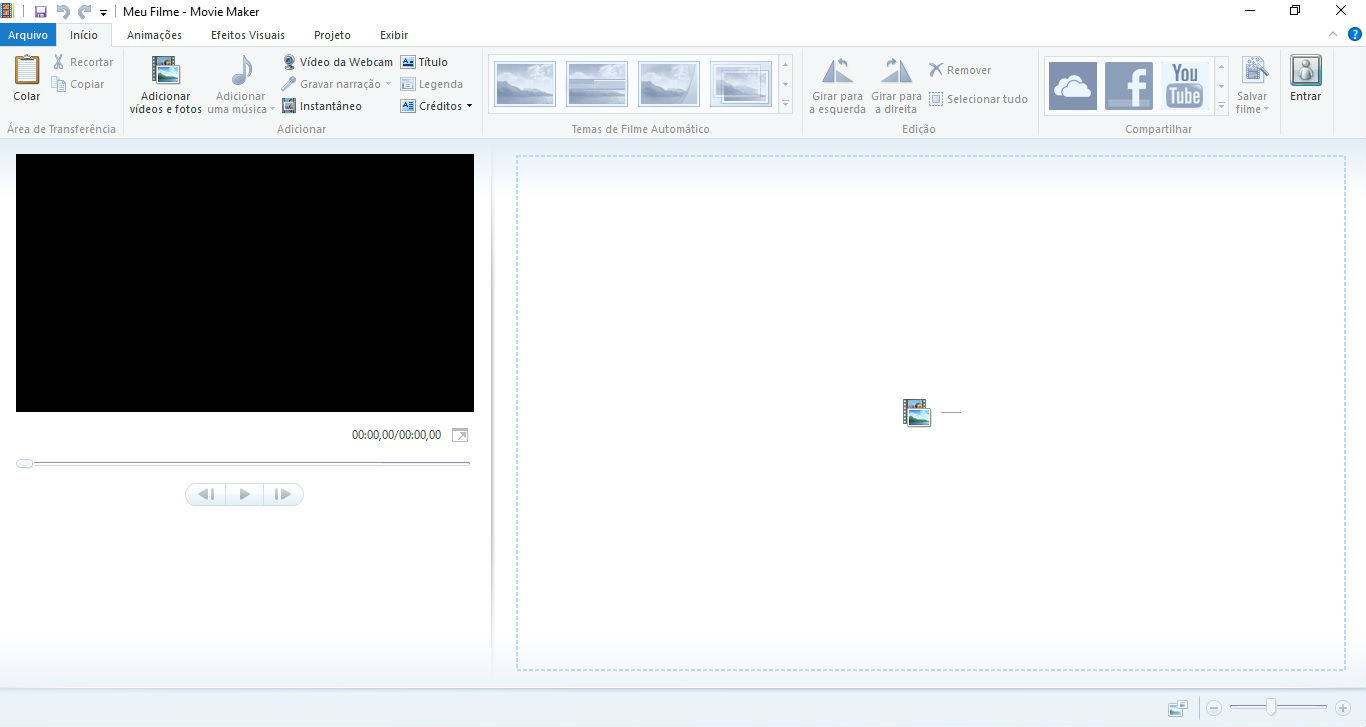
\includegraphics[scale=0.4]{1.jpg}
\end{figure}

\newpage

\section{Importando suas fotos e músicas:}
\begin{enumerate}
\item Do lado superior esquerdo da tela, clique em \textbf{Adicionar fotos e vídeos}. Busque na pasta do projeto as imagens que separou e clique em \textbf{Importar}.
\item No lado direito da tela você formará uma coleção com os arquivos que vai usar no projeto.
\end{enumerate}

\begin{figure}[h!]
\centering
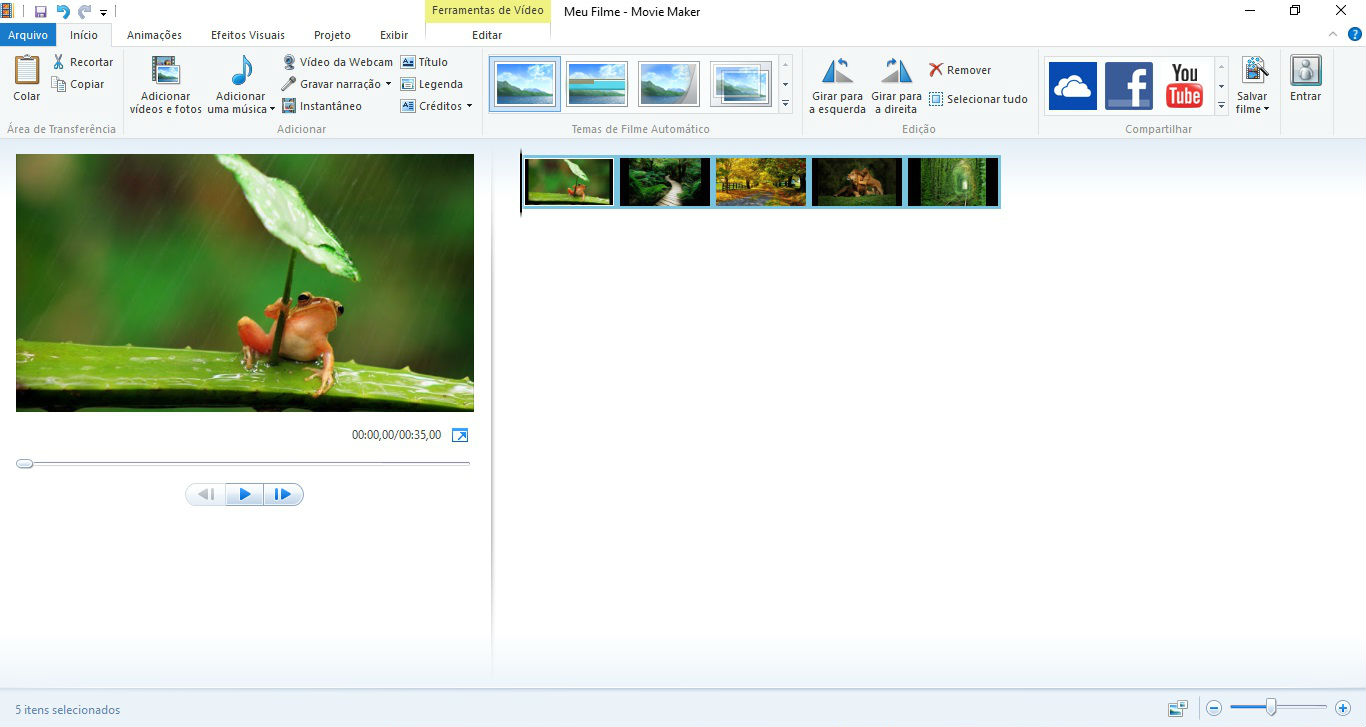
\includegraphics[scale=0.4]{2.jpg}
\end{figure}

\newpage

\section{Montando o storyboard:}
\begin{enumerate}
\item Para montar o storyboard é simples: Basta ir adicionando as fotos
\item Faça o mesmo com as demais fotos e vídeos lembrando sempre da ordem que deseja que apareçam em seu projeto;
\item Se deseja ter uma idéia de como ficará, selecione a primeira imagem no storyboard e na tela ao lado clique no play.
\end{enumerate}

\begin{figure}[h!]
\centering
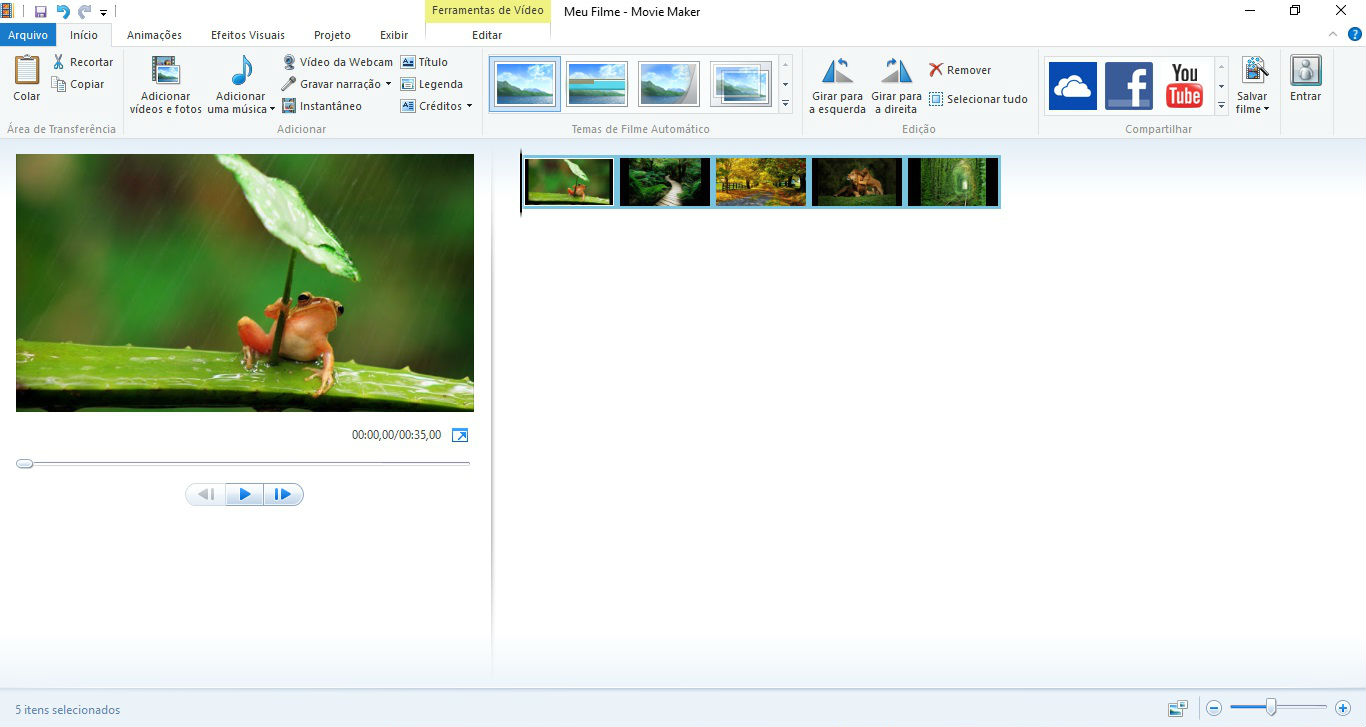
\includegraphics[scale=0.4]{2.jpg}
\end{figure}

\newpage

\section{Inserindo uma música:}
\begin{enumerate}
\item Para adicionar músicas basta clicar em \textbf{Adicionar uma música} e selecionar
uma desejada;
\item Note que outra aba abrirá, em que você possa editar a música da maneira
que o seu filme necessite.
\end{enumerate}

\begin{figure}[h!]
\centering
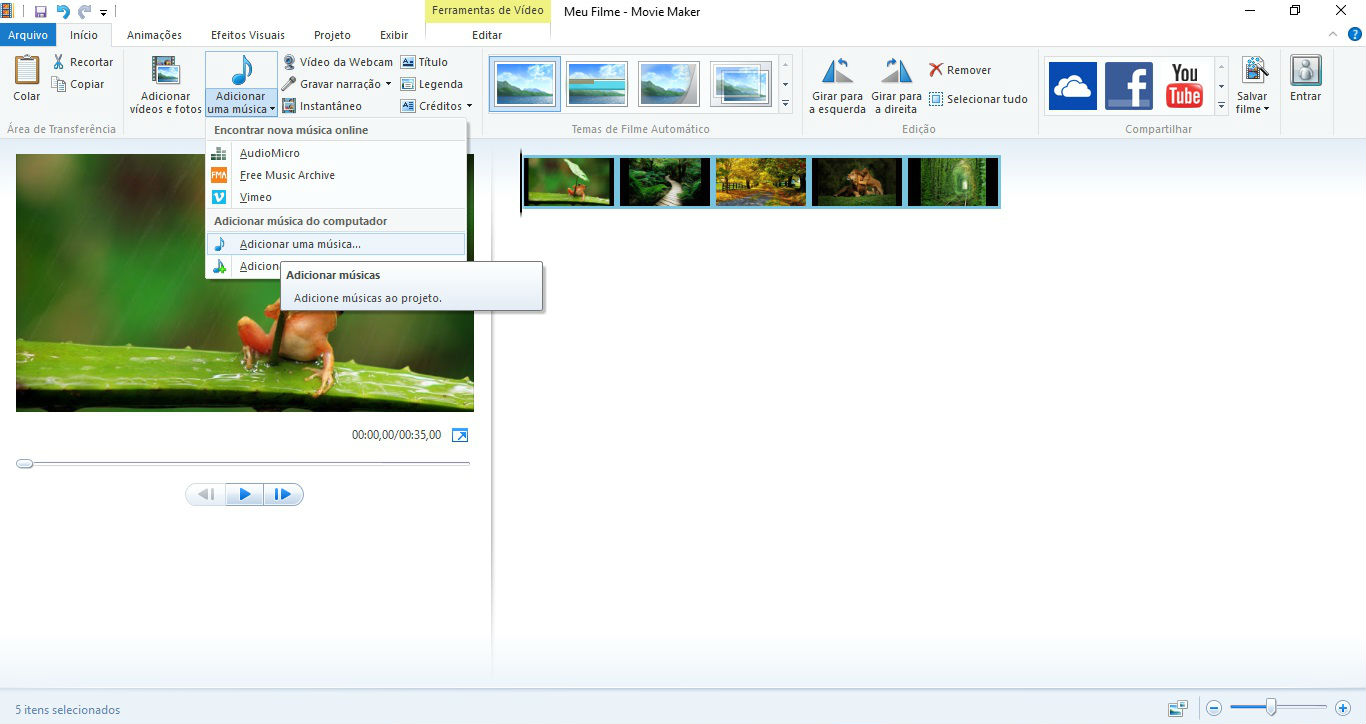
\includegraphics[scale=0.4]{3.jpg}
\end{figure}

\newpage

\section{Inserindo textos:}
\begin{enumerate}
\item Para adicionar textos, clique em \textbf{Início} e depois em \textbf{Legendas};
\item Uma aba de edição abrirá em que você poderá editar usa legenda, tipo fonte e tamanho;
\end{enumerate}

\begin{figure}[h!]
\centering
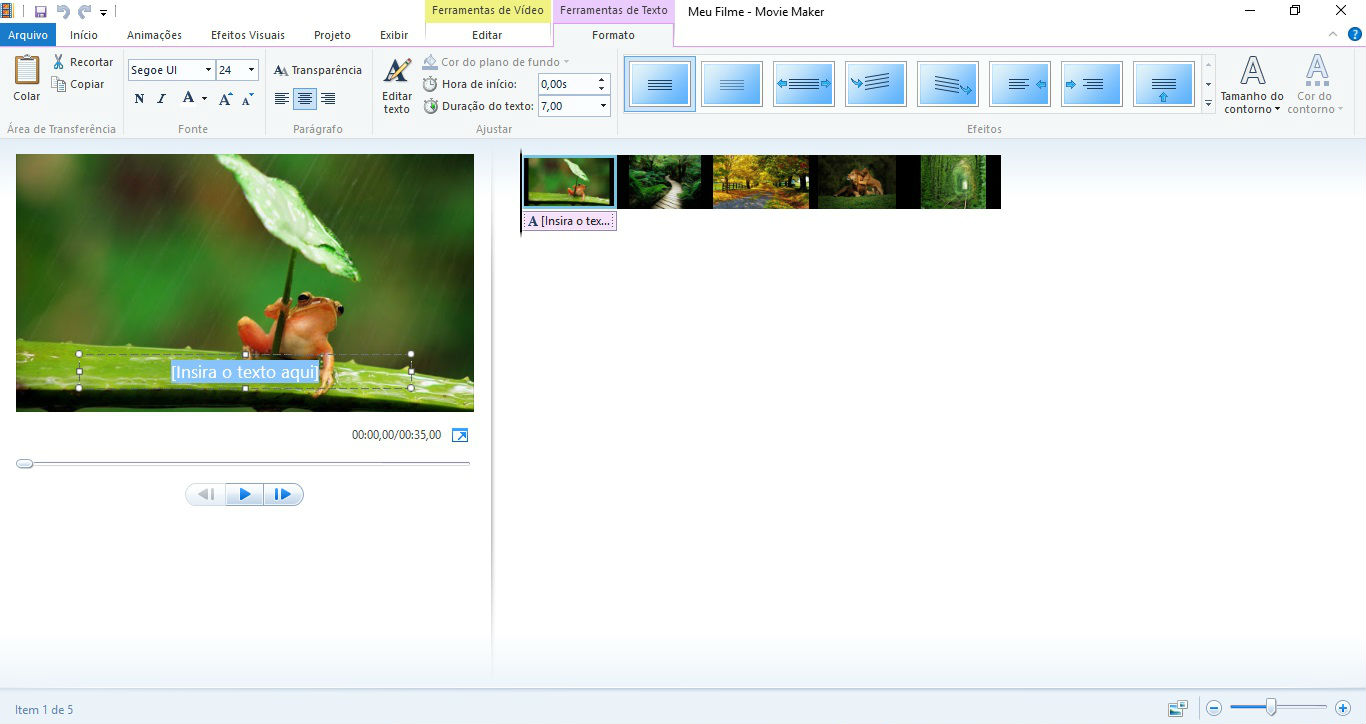
\includegraphics[scale=0.4]{4.jpg}
\end{figure}

\newpage

\section{Inserindo efeitos especiais:}
\begin{enumerate}
\item Para inserir um efeito, ou vários, em seu filme, clique na aba \textbf{Efeitos Visuais} na barra de ferramentas. Lá aparecerá diversos efeitos que você poderá aplicar em suas fotos;
\item Escolha o efeito que mais combina com o seu filme, clique nele e arraste até o storyboard, dentro do quadrado com uma estrela dentro, no canto inferior
esquerdo. Pronto! Solte o efeito e aperte o play para visualizar;
\item Faça isso em todas as imagens do storyboard. 
\item \textbf{Dica:} Você pode escolher um efeito diferente para cada quadrado!
\end{enumerate}

\begin{figure}[h!]
\centering
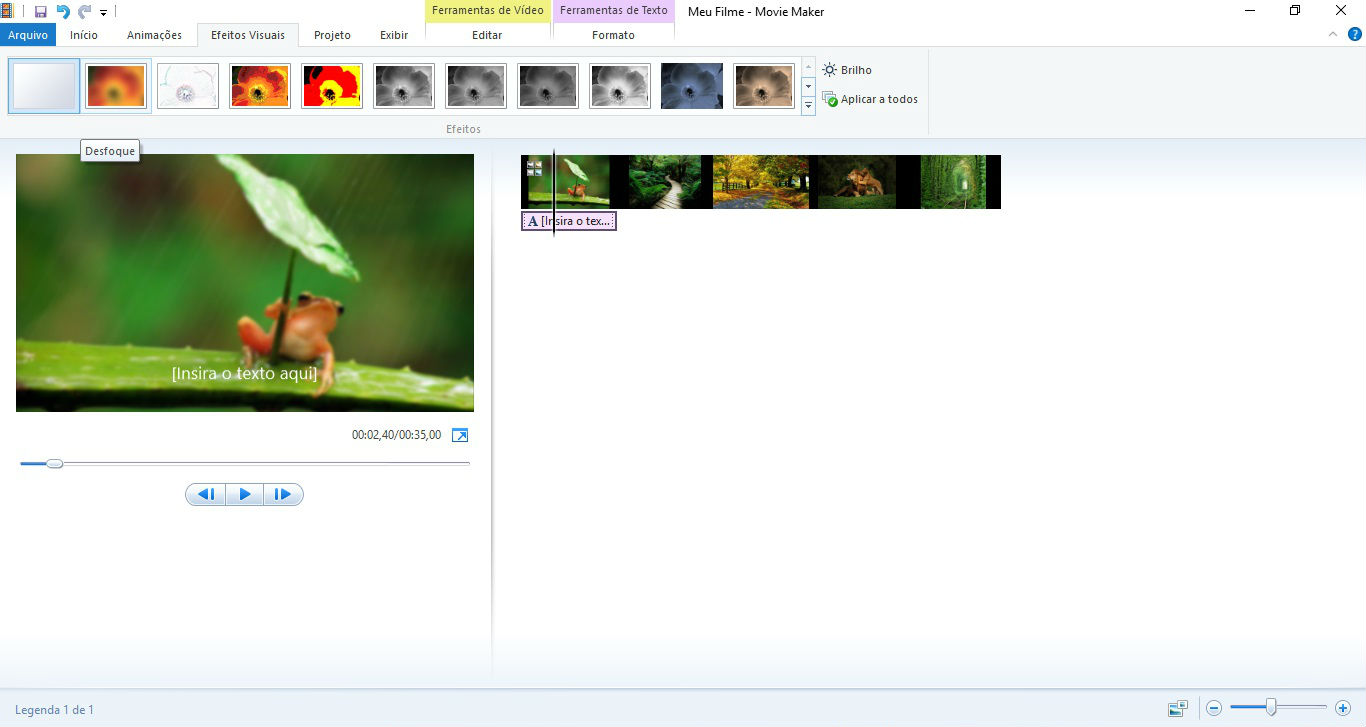
\includegraphics[scale=0.4]{5.jpg}
\end{figure}

\newpage

\section{Inserindo animações de transições:}
\begin{enumerate}
\item Efeitos de transição são os efeitos que aparecerão no começo da aparição da sua imagem;
\item Para adicionar efeitos de transição basta clicar em \textbf{Animações} na barra de ferramentas selecionar o efeito desejado para iniciar a apresentação de cada imagem. Note também que para casa transição existe um tempo de duração que você poderá alterar se necessário;
\item Assim como na adição de efeitos nas imagens, você pode escolher em aplicar o efeito de transição em todas as imagens ou somente na selecionada.
\end{enumerate}

\begin{figure}[h!]
\centering
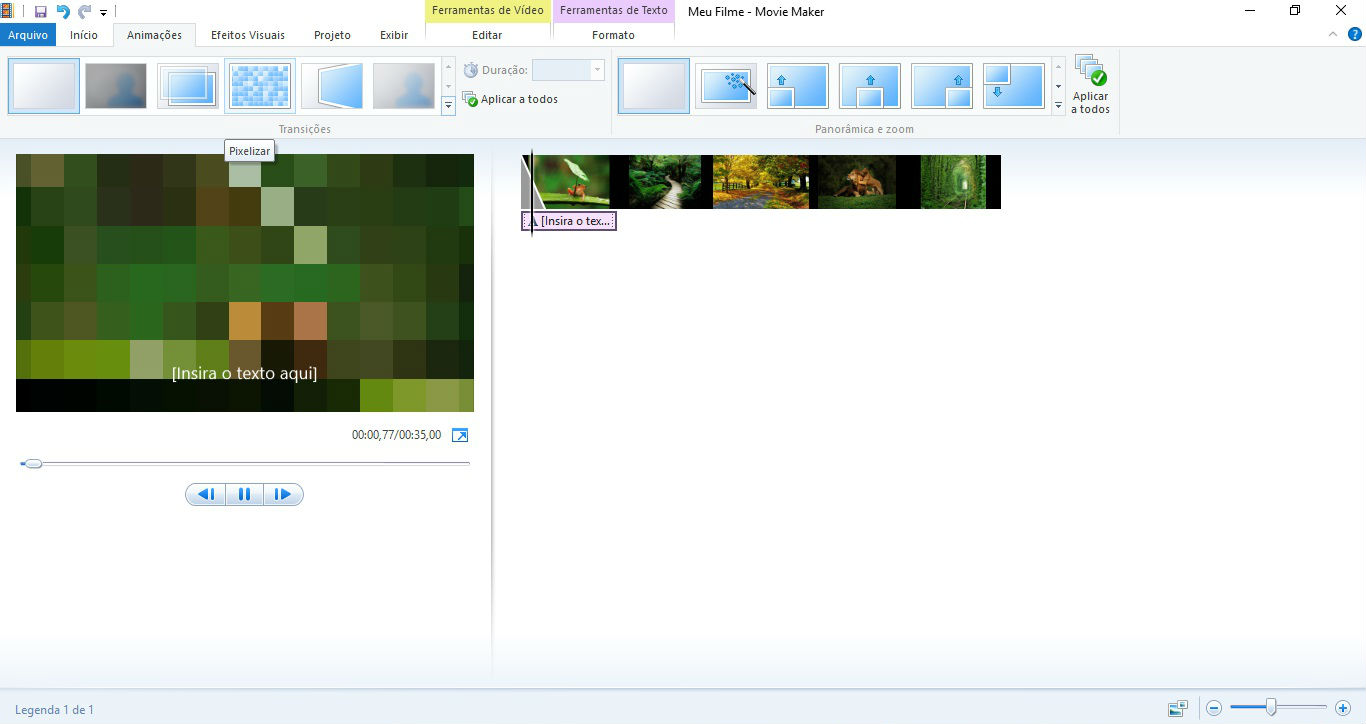
\includegraphics[scale=0.4]{6.jpg}
\end{figure}

\newpage

\section{Salve o projeto como filme:}
\begin{enumerate}
\item Você já salvou o projeto, agora é hora de salvar o filme;
\item No menu superior clique em \textbf{Arquivo}. Escolha a opção \textbf{Salvar arquivo de filme};
\item Escolha a opção salvar em \textbf{Meu Compputador}. Clique para
avançar;
\item Insira o nome do filme e escolha aonde quer salvar dentro do seu computador. Clique para avançar;
\item Escolha a opção \textbf{Melhor qualidade para reprodução no computador}. Clique para avançar;
\end{enumerate}

\begin{figure}[h!]
\centering
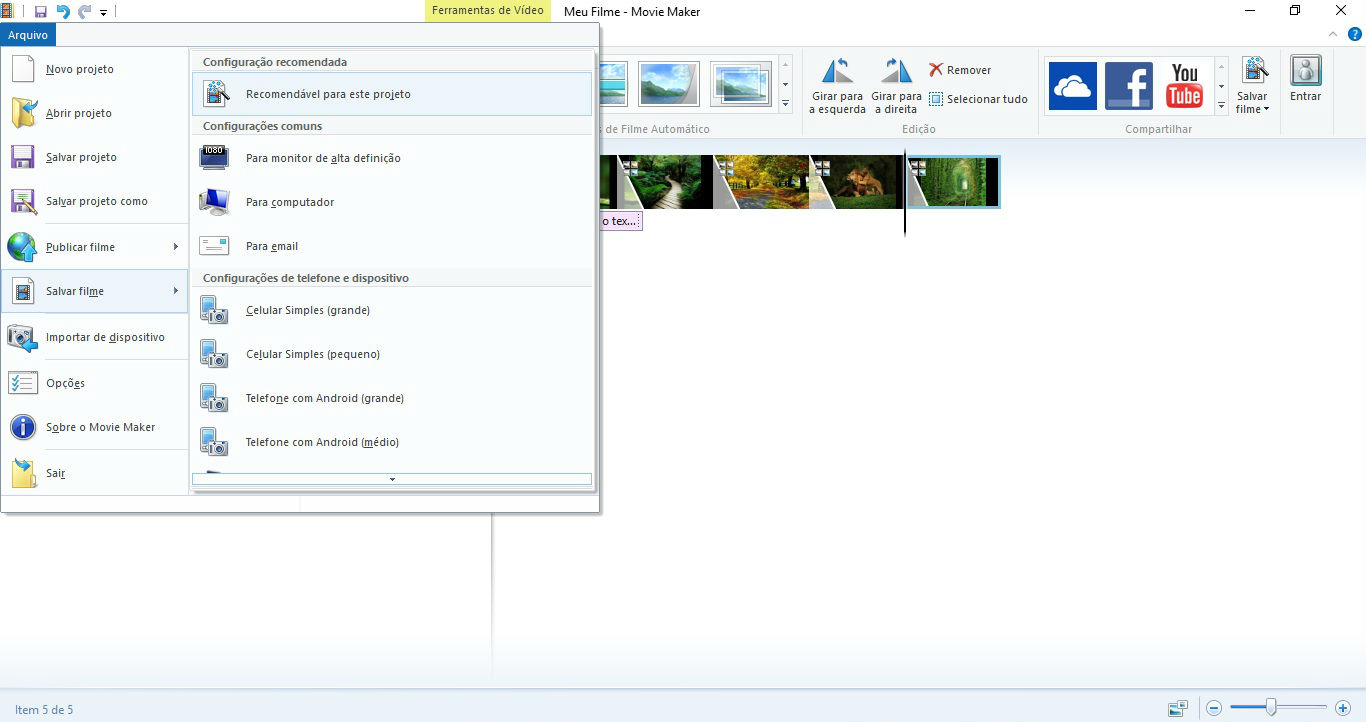
\includegraphics[scale=0.4]{7.jpg}
\end{figure}

}
\end{document}